\section{Appendix}\label{sec:appendix}
\begin{lstlisting}[language=json, caption={LabelStudio JSON format.}, label={A1}, captionpos=b, basicstyle=\footnotesize]
{
    "id": 1585,
    "annotations": [
      {
        "id": 1520,
        "completed_by": 1,
        "result": [
          {
            "original_width": 500,
            "original_height": 384,
            "image_rotation": 0,
            "value": {
              "x": 1.1999999999999997,
              "y": 1.0416666666666665,
              "width": 97.59999999999995,
              "height": 97.13541666666664,
              "rotation": 0,
              "rectanglelabels": [
                "Lepidoptera"
              ]
            },
            "id": "G5K3NFjz3X",
            "from_name": "label",
            "to_name": "image",
            "type": "rectanglelabels",
            "origin": "manual"
          }
        ],
        "was_cancelled": false,
        "ground_truth": false,
        "created_at": "2022-02-12T11:27:48.299000Z",
        "updated_at": "2022-02-12T18:01:40.688292Z",
        "lead_time": 14.013,
        "prediction": {},
        "result_count": 0,
        "task": 1585,
        "parent_prediction": null,
        "parent_annotation": null
      }
    ],
    "drafts": [],
    "predictions": [],
    "data": {
      "image": "IMAGE_NAME"
    },
    "meta": {},
    "created_at": "2022-02-11T20:01:40.340238Z",
    "updated_at": "2022-02-12T18:01:40.721007Z",
    "project": 2
  }
\end{lstlisting}


\begin{figure}[!ht]
    \centering
    \begin{minipage}{\textwidth}
        \centering
        \rotatebox[origin=c]{90}{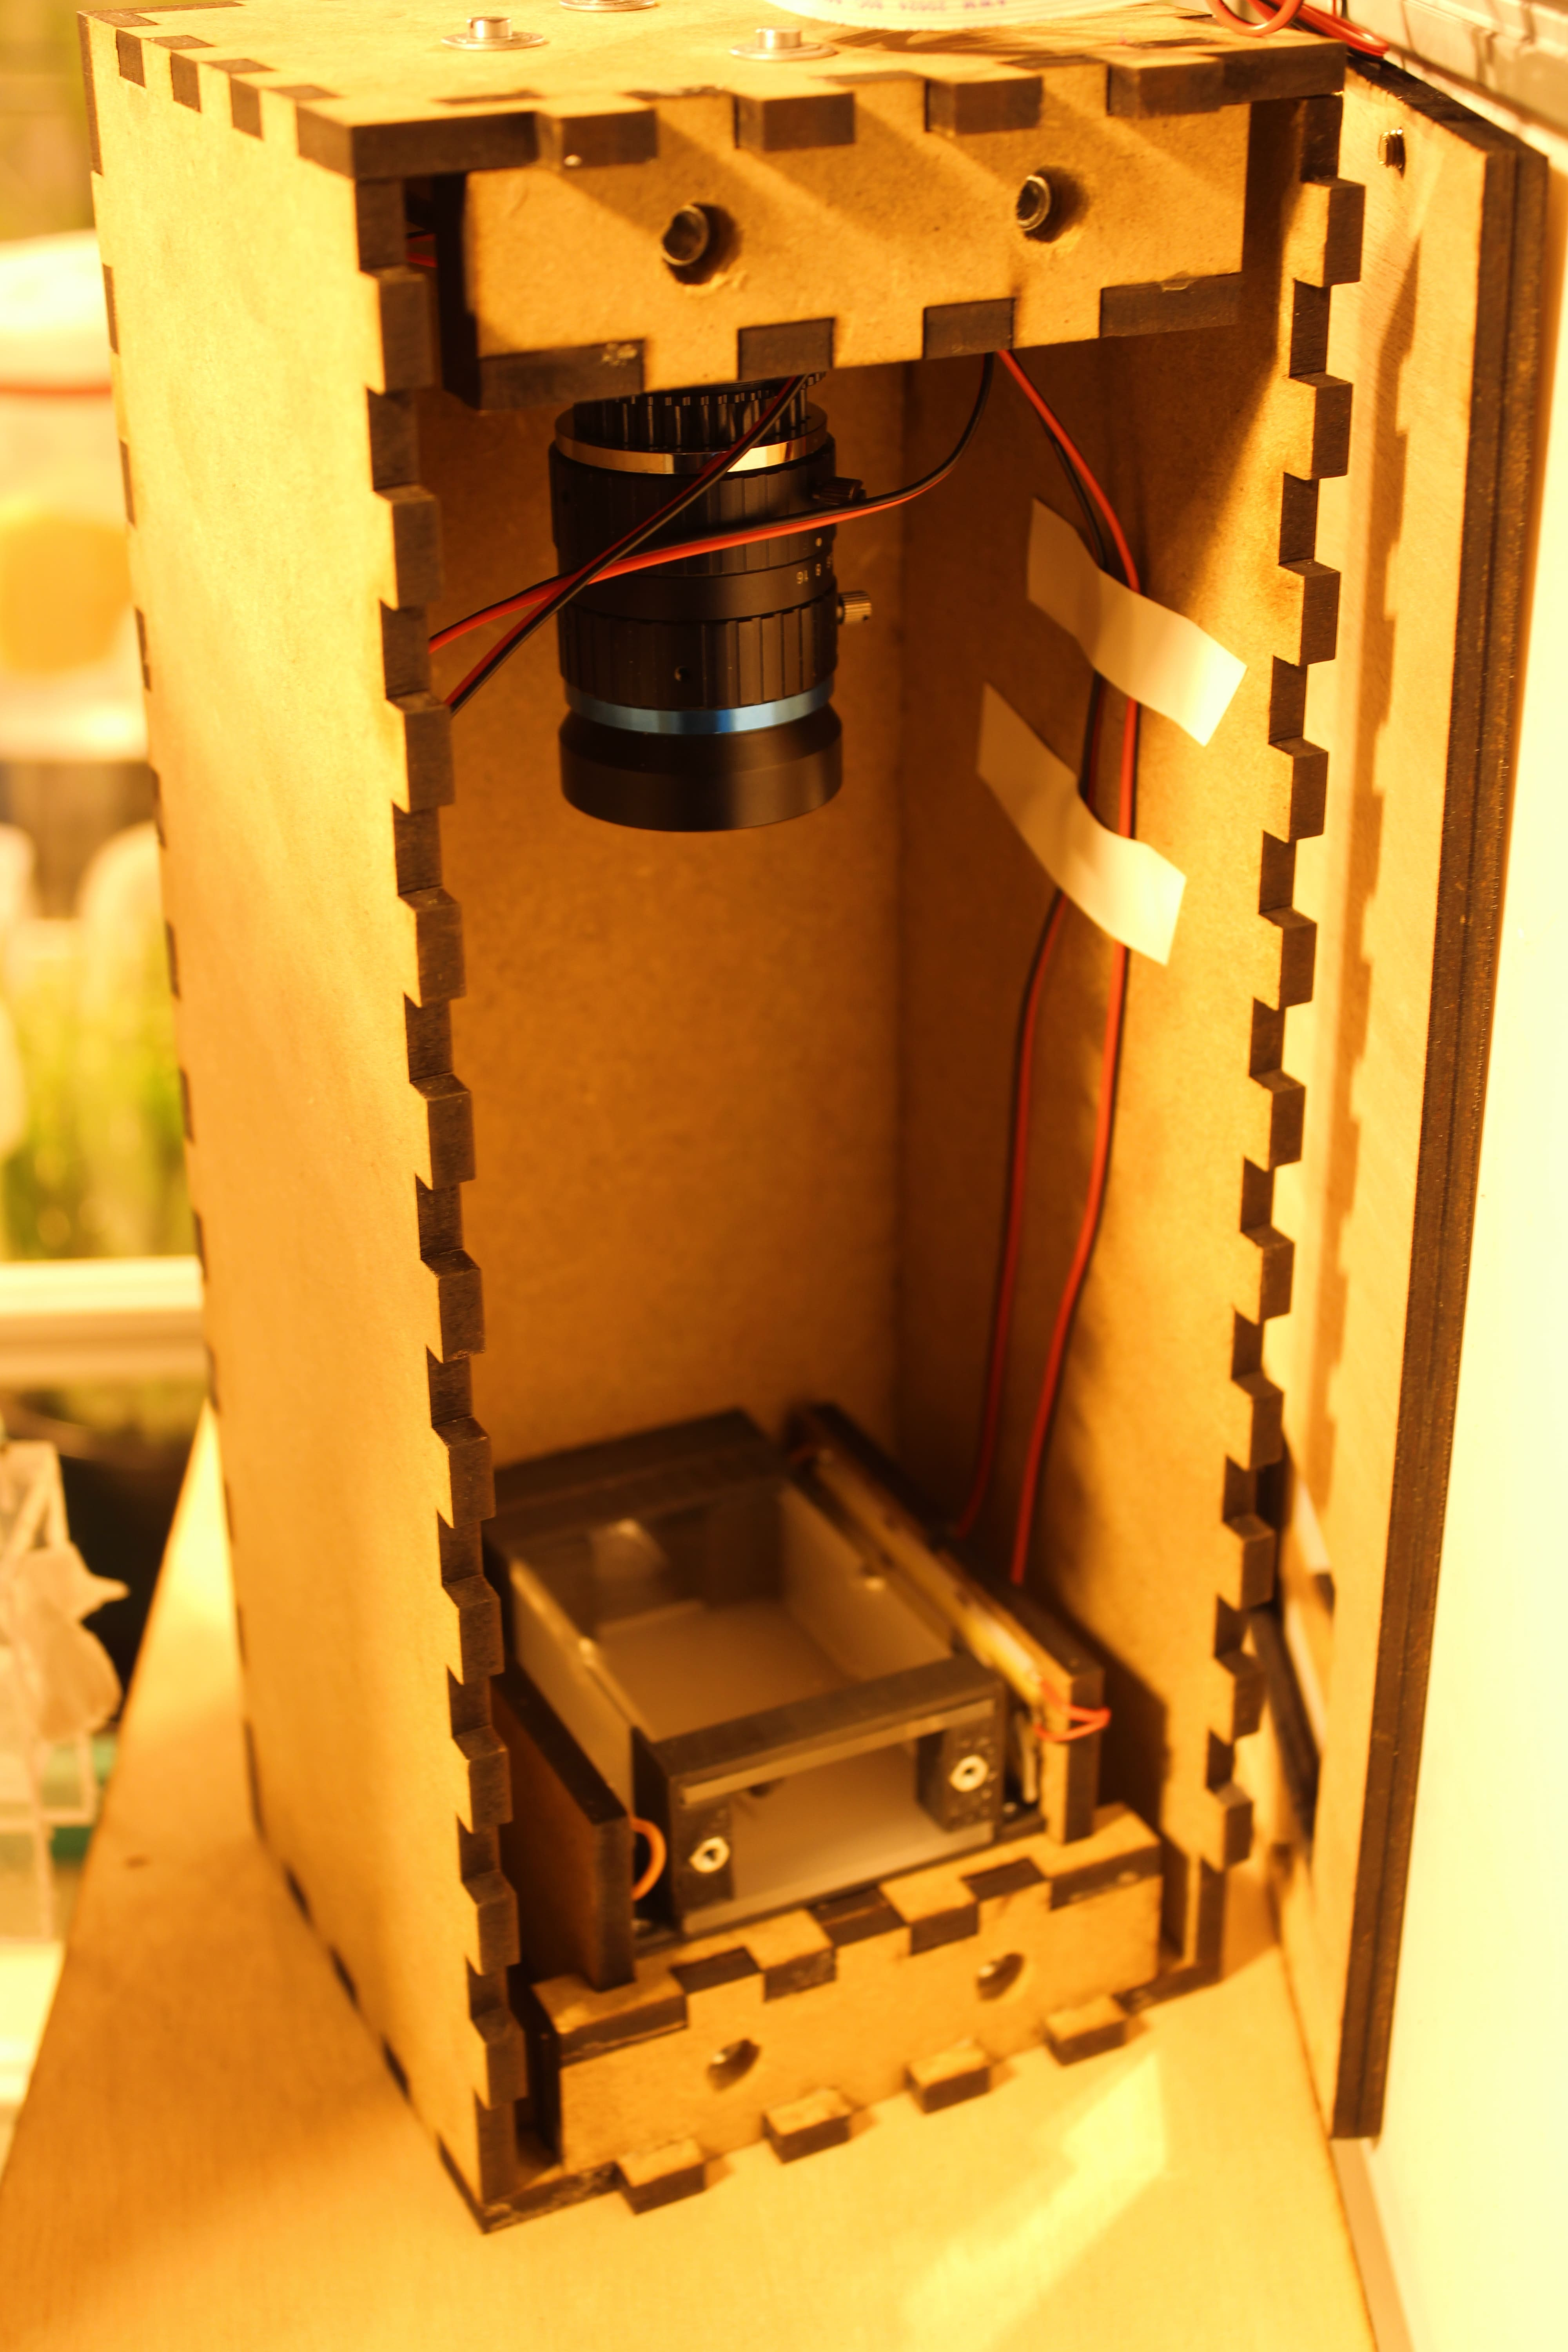
\includegraphics[width=\textwidth,keepaspectratio]{src/images/camera.JPG}}
        \caption{Camera module of the \textit{KInsecta} device. High resolution camera lens on top and a light source triggered by a light barrier on bottom.}
        \label{fig:camera}
    \end{minipage}
\end{figure}
\begin{figure}[!ht]
    \begin{minipage}{\textwidth}
        \centering
        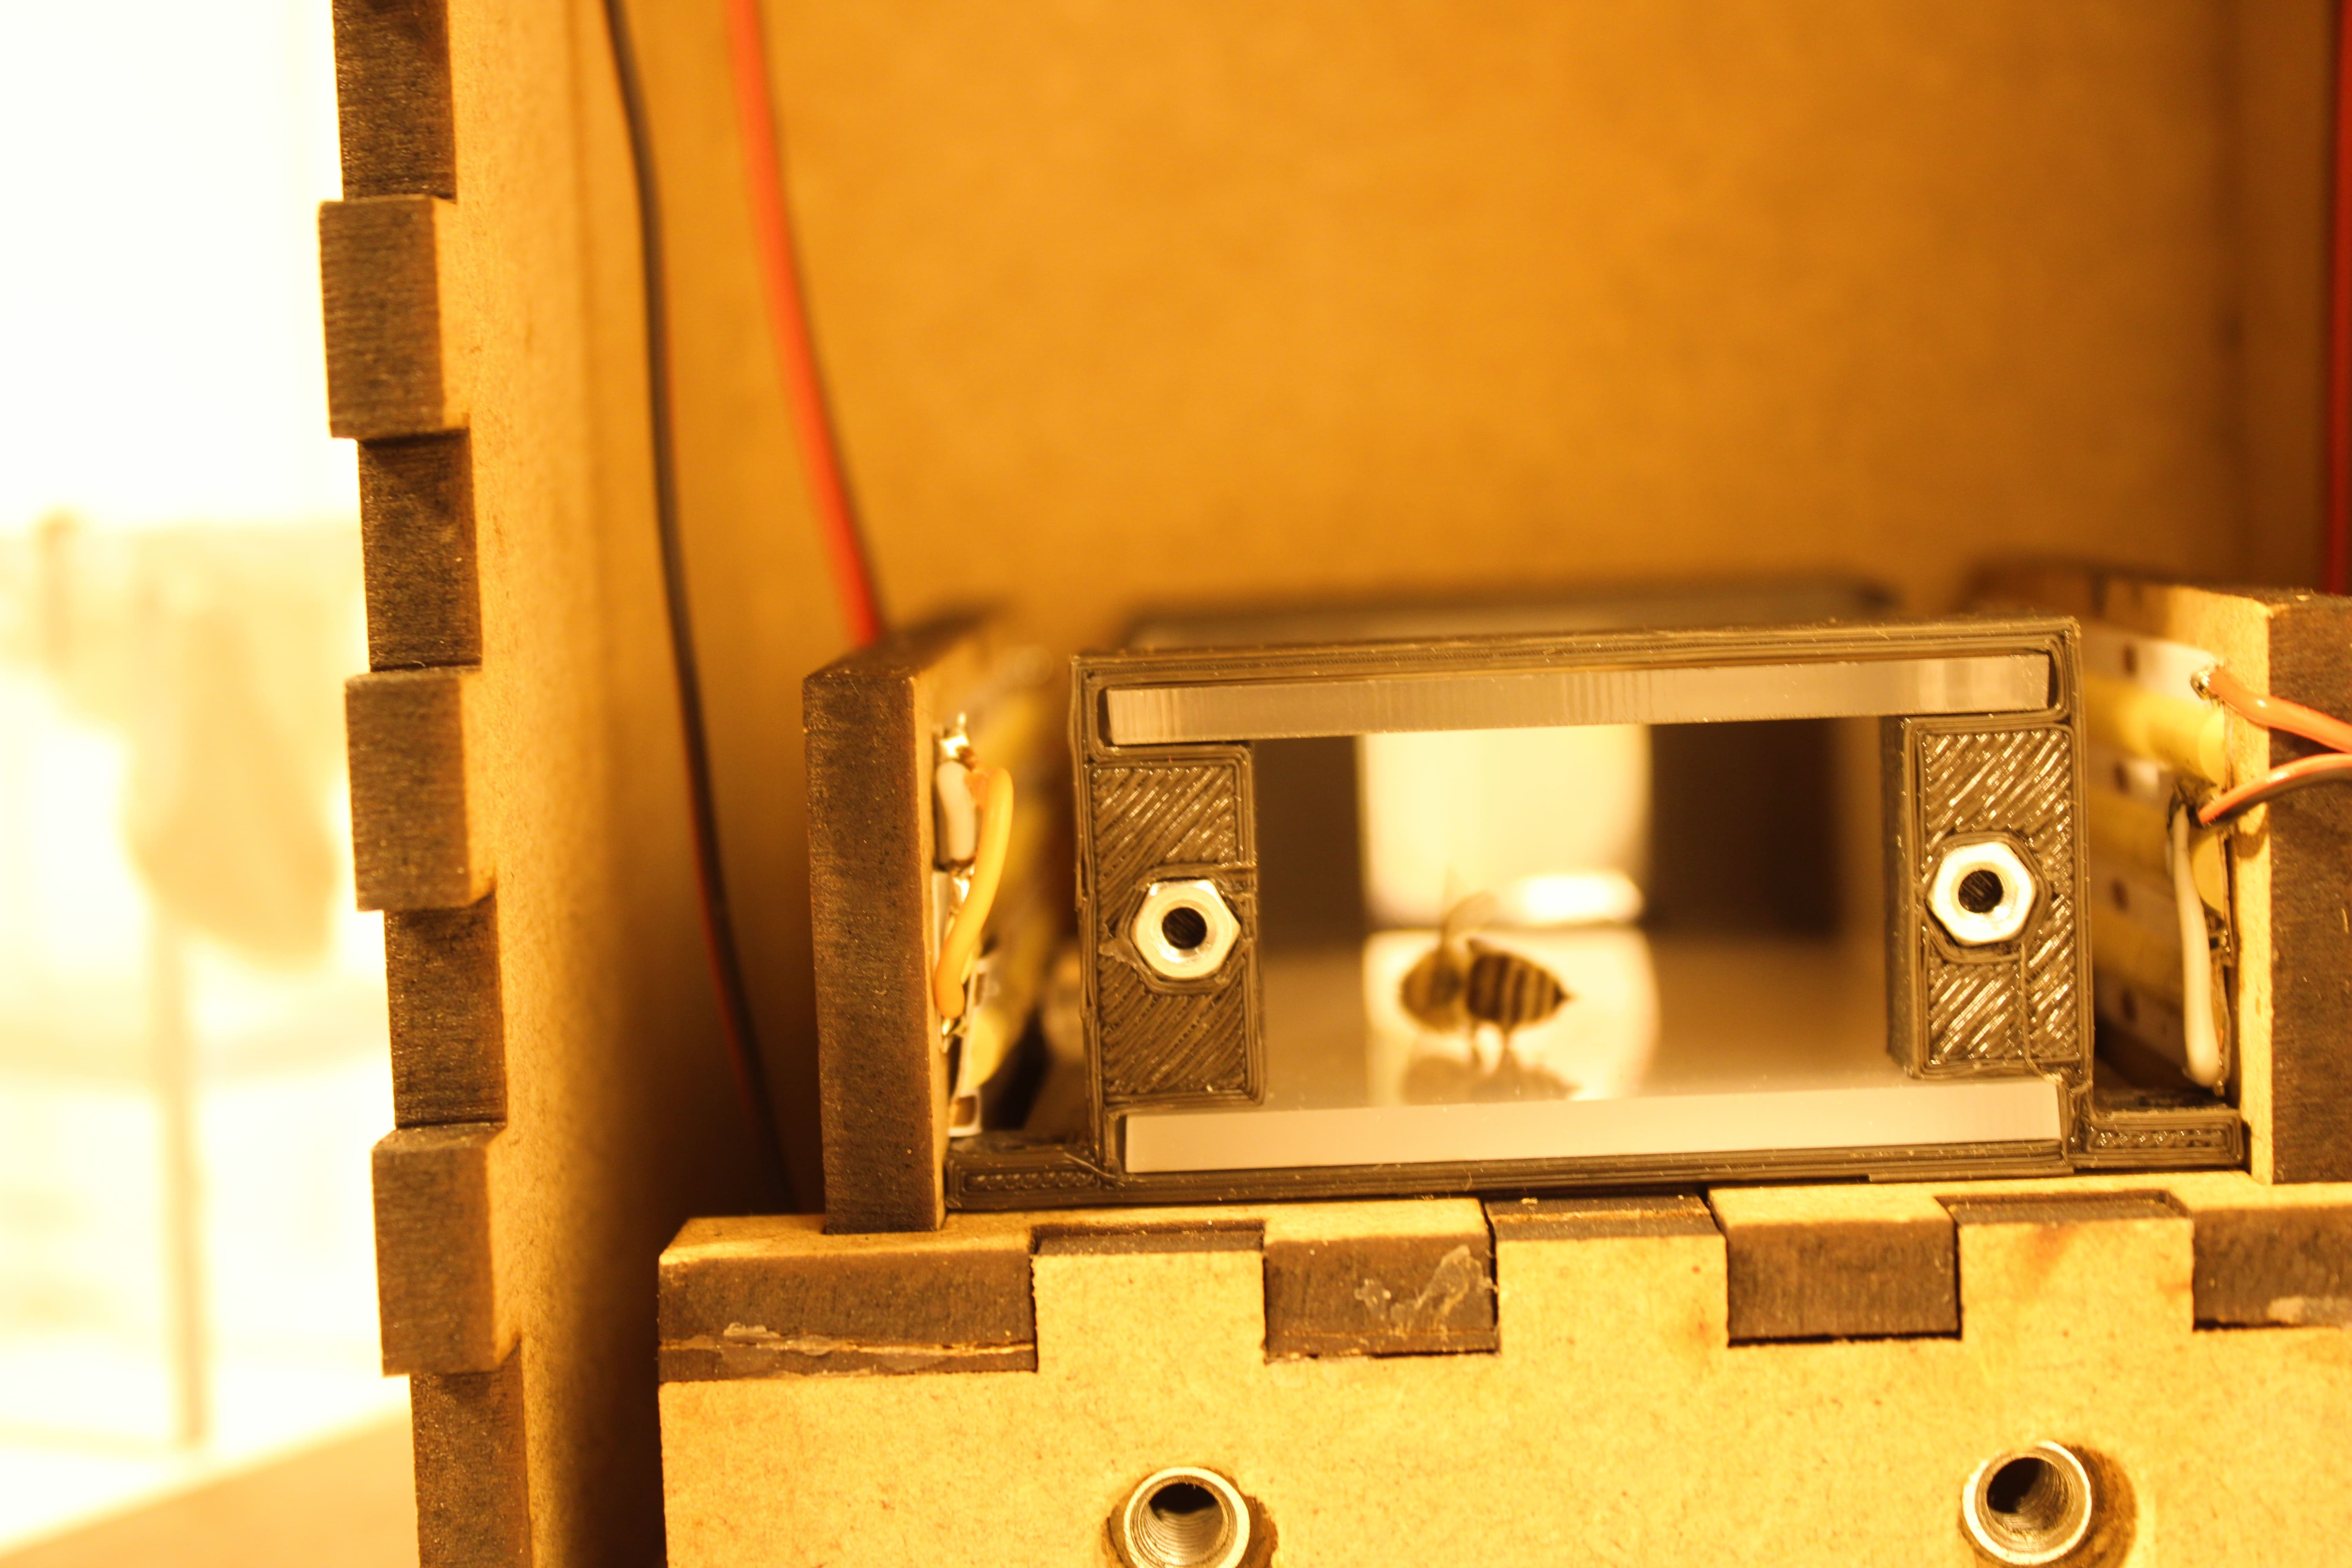
\includegraphics[width=\textwidth,keepaspectratio]{src/images/camera-look-through.JPG}
        \caption{Look through the passage an insect needs to walk through to get recorded.}
        \label{fig:camera-look-through}
    \end{minipage}
\end{figure}
\begin{figure}[!ht]
    \begin{minipage}{\textwidth}
        \centering
        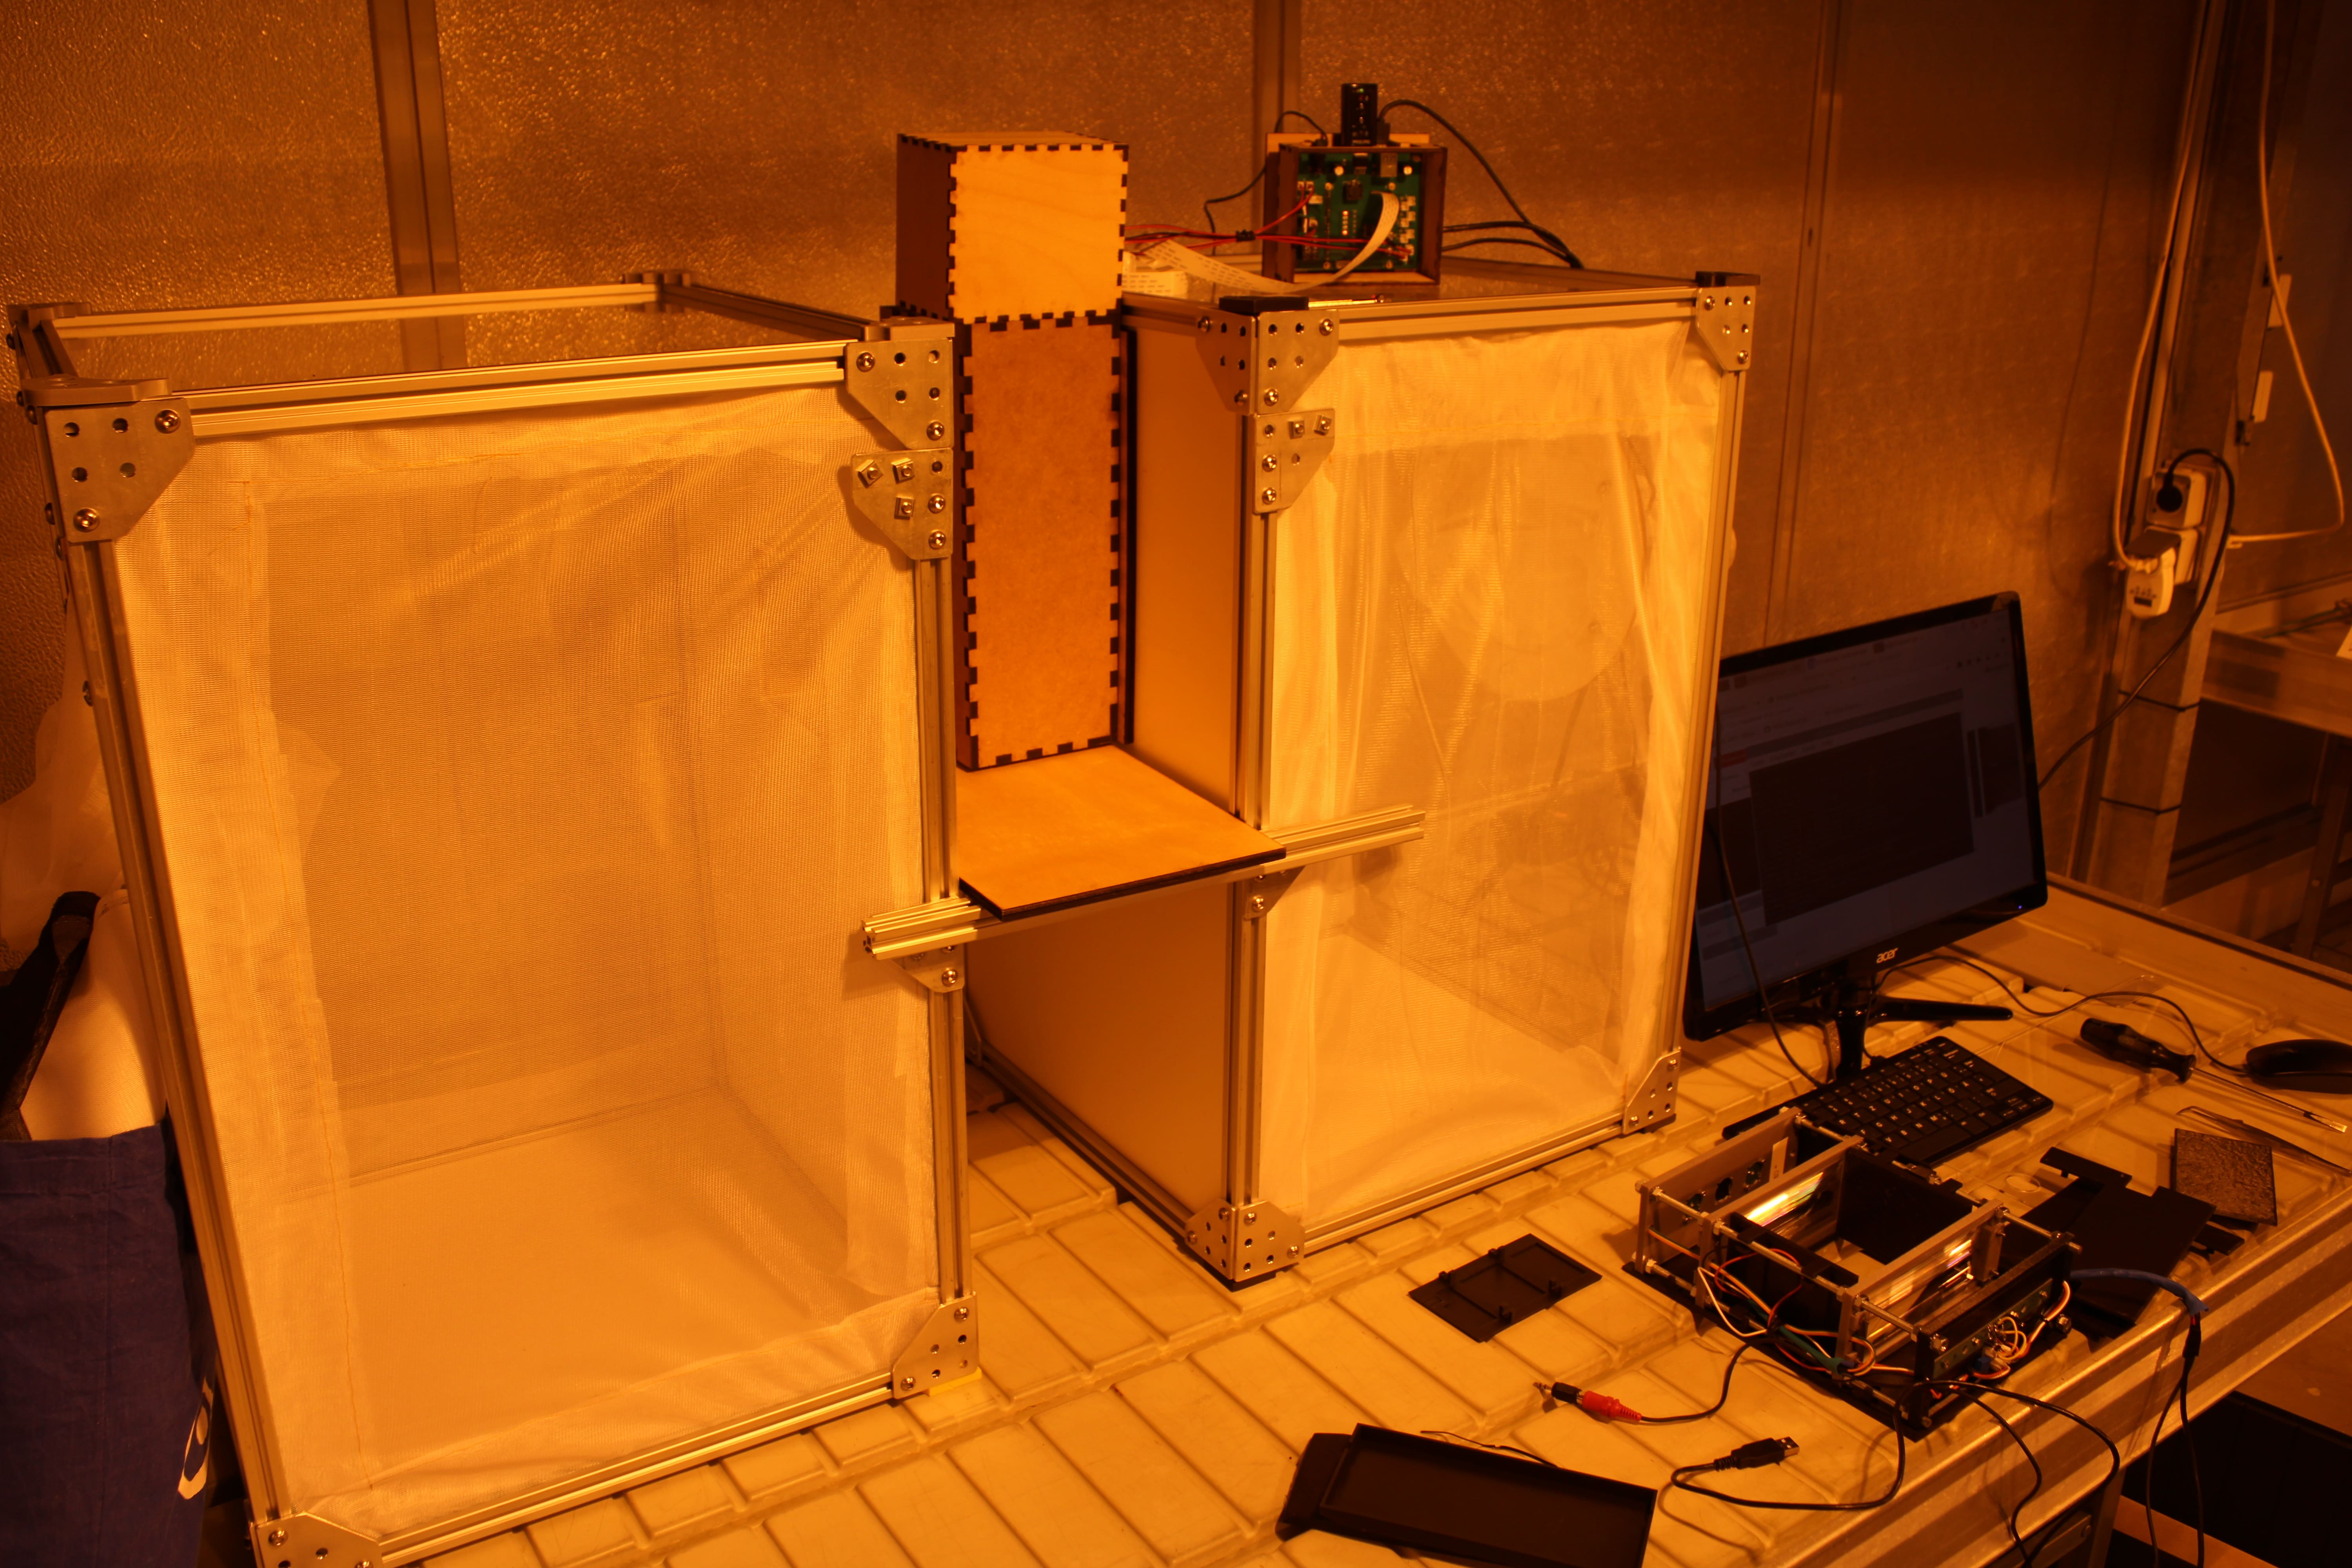
\includegraphics[width=\textwidth]{src/images/experimental-setup.JPG}
        \caption{An experimental setup of the \textit{KInsecta} device. Two containers, which will later contain specific insect species, connected with a passage leading through different setups for different sensors (wooden boxes). On the table lies the detached \textit{WindBeat} sensor. Next to it a monitor and keyboard are connected to the \textit{RaspberryPi} on top of the right box.}
        \label{fig:experiment-setup}
    \end{minipage}
\end{figure}

\begin{figure}[!ht]
    \centering
    \includegraphics[width=\textwidth]{src/images/dataset-representation.eps}
    \caption{Representation of the here used data set displaying the five insect orders. It is easy to notice that all vary in quality as well as focus and coverage of important surface areas. Especially Hemiptera and Formicidae are difficult for Localization of individual insects due to the fact that they mostly appear in herds of multiple insects.}
    \label{fig:dataset-overview}
\end{figure}

\begin{figure}[!ht]
    \centering
    \includegraphics[width=\textwidth,keepaspectratio]{src/images/augmentation-samples.eps}
    \caption{Visualization of different augmentation methods, from top down as listed in "\nameref{subsec:augmentation}".}
    \label{fig:augmentation-samples}
\end{figure}


\begin{table}[!ht]
    \centering
    \begin{tabular}{|c|c|}
        \hline
        \textbf{Parameter} & \textbf{Options} \\
        \hline
        Learning Rate & $\{1^{-4}, 5^{-4}, 1^{-3}, 5^{-3}, 1^{-2}\}$\\
        \hline
        Regualrization Factor & $\{1^{-4}, 5^{-4}, 1^{-3}, 5^{-3}, 1^{-2}\}$\\
        \hline
    \end{tabular}
    \caption{Available parameters for regression HPO.}
    \label{fig:reg-hp-table}
\end{table}
\begin{table}[!ht]
    \centering
    \begin{tabular}{|c|c|}
        \hline
        \textbf{Parameter} & \textbf{Options} \\
        \hline
        Learning Rate & $\{1^{-4}, 5^{-4}, 1^{-3}, 5^{-3}, 1^{-2}\}$\\
        \hline
        Regualrization Factor & $\{1^{-4}, 5^{-4}, 1^{-3}, 5^{-3}, 1^{-2}\}$\\
        \hline
        Frozen Layers & $\{$0: All, 1: half, 2: None$\}$\\
        \hline
    \end{tabular}
    \caption{Available parameters for HPO of classification models.}
    \label{fig:clf-hp-table}
\end{table}

\begin{figure}
    \centering
    \begin{minipage}{.45\textwidth}
    \includegraphics[width=\textwidth]{src/images/ridge-svm-two-stage-model-confusion.png}
    \end{minipage}
    \hfill
    \begin{minipage}{.45\textwidth}
    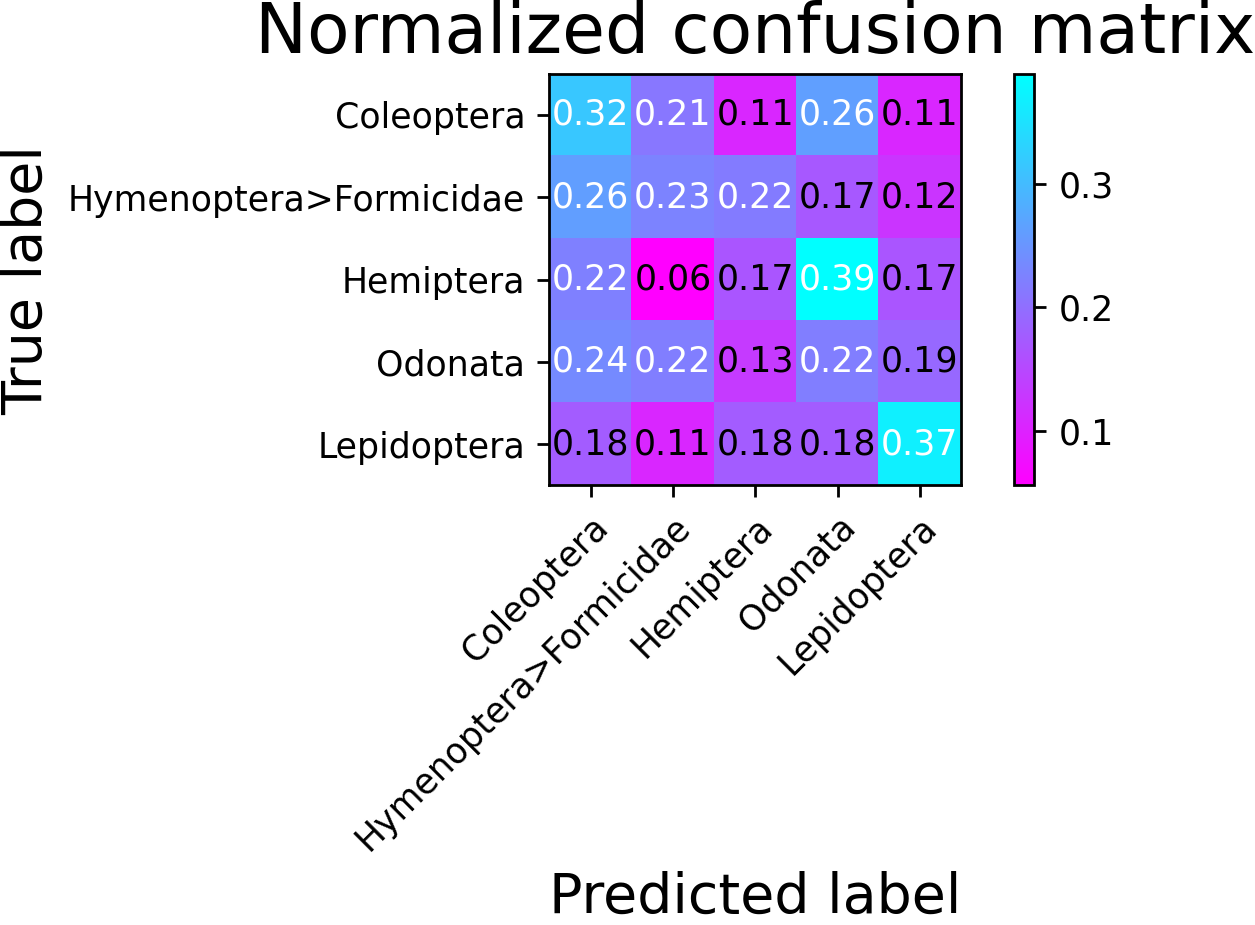
\includegraphics[width=\textwidth]{src/images/pca-400-ridge-svm-two-stage-model-confusion.png}
    \end{minipage}
    \caption{Confusion matrices for conventional methods based on the validation set. Left predictions performed with a model using $\text{PCA}_{100}$, right $\text{PCA}_{400}$. No distinctive classification for both cases. The predictions seem randomly distributed. Most cells contain values $\approx0.2$, which is the same value as a random guess.}
    \label{fig:conventional-confusions}
\end{figure}

%% Results
\begin{figure}[!ht]
    \centering
    \begin{minipage}{.45\textwidth}
    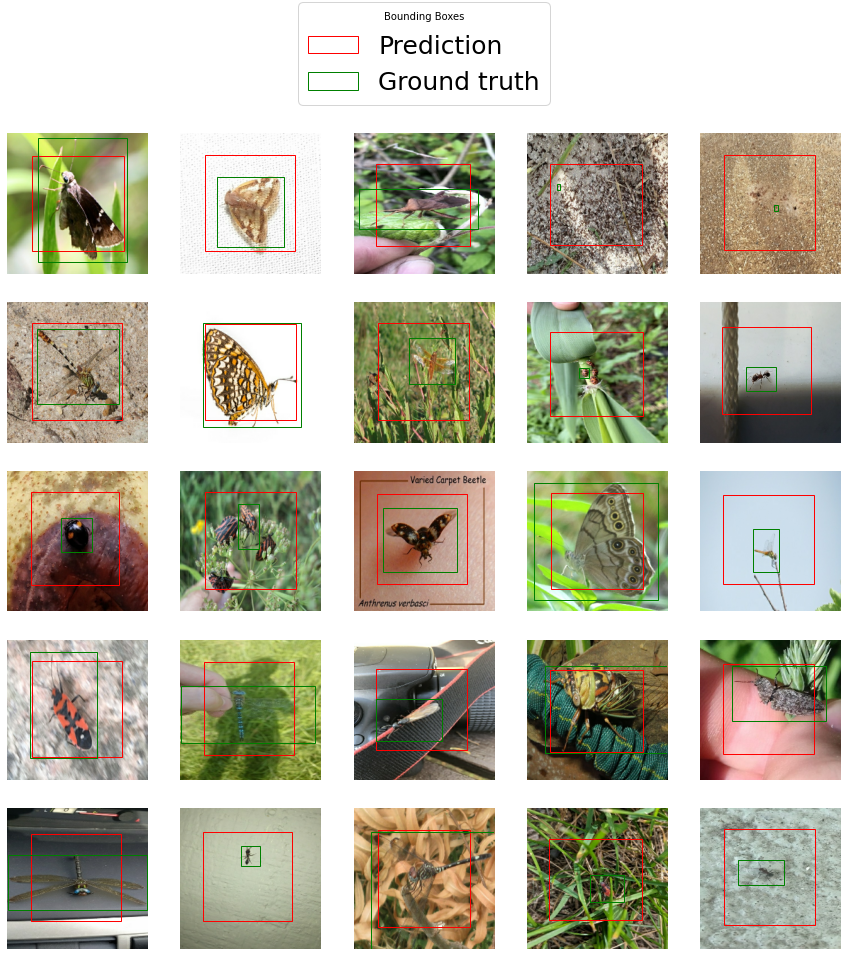
\includegraphics[width=\textwidth]{src/images/regression-mobilenet-raw.png}
    \end{minipage}
    \hfill
    \begin{minipage}{.45\textwidth}
    \includegraphics[width=\textwidth]{src/images/regression-mobilenet-augmented.png}
    \end{minipage}
    \caption{BB predictions on validation set of final models after HPO, using MobileNet as backbone. Left contains predictions from a model trained on the raw training data set. The predictions seem to be bound to a fixed location. Right, predictions performed with a MobileNet backbone optimized while training on the augmented training data set. Leading to a higher variance in BB locations and dimensions.}
    \label{fig:regression-samples-mobilenet}
\end{figure}

% TESTS
\begin{landscape}
\begin{table}[!ht]
    \centering
    \begin{tabular}{|l|l|c|c|c|c|c|}
    \hline
         \textbf{Backbone} & \textbf{Data set} & \textbf{GIoU} & \textbf{RMSE} & \textbf{Learning Rate} & $\mybold{\alpha}$
         & \textbf{HPO Time}\\

    \hline
        INet & Raw & $0.3838$ & $25.9176$ & $0.005$ & $0.0005$ & 2h 42m\\
    \hline
        MobileNet & Raw & $0.3877$ & $25.3727$ & $0.01$ & $0.0001$ & 7h 30m\\
    \hline
        VGG-16 & Raw & $0.0525$ & $24.2184$ & $0.001$ & $0.01$ & 11h 20m\\
    \hline
    \hline
        INet & Augmented & $0.3670$ & $26.3442$ & $0.01$ & $0.01$ & 11h 15m\\
    \hline
        \textbf{MobileNet}
        & \textbf{Augmented}
        & $\mybold{0.5602}$
        & $\mybold{17.0061}$
        & $\mybold{0.0005}$
        & $\mybold{0.0001}$
        & \textbf{19h 15m}\\
    \hline
        VGG-16 & Augmented & $-0.4000$ & $40.7438$ & $0.0001$ & $0.001$ & 22h\\
    \hline
    \end{tabular}
    \caption{HPO results for BBReg trained on a raw data set with sample of shape \eqref{eq:regression-sample} ("Raw") and an augmented version of it ("Augmented").}
    \label{fig:two-stage-regression-results}
\end{table}
\begin{table}[!ht]
    \centering
    \begin{tabular}{|l|l|c|c|c|c|c|c|}
        \hline
         \textbf{Backbone} & \textbf{Data set} &  \textbf{Accuracy} & \textbf{F1} & \textbf{Learning Rate} & $\mybold{\alpha}$
         & \textbf{Frozen Blocks} & \textbf{HPO Time}\\
        \hline
        INet &
        Raw &
        $0.6422$ &
        $0.7793$ &
        $0.005$ &
        $0.0001$ &
        0 &
        2h 30
        \\
        \hline
        \textbf{MobileNet} &
        \textbf{Raw} &
        $\mybold{0.8511}$ &
        $\mybold{0.8462}$ &
        $\mybold{0.01}$ &
        $\mybold{0.001}$ &
        \textbf{1} &
        \textbf{6h 50m}
        \\
        \hline
        VGG-16 &
        Raw &
        $0.8467$ &
        $0.8439$ &
        $0.001$ &
        $0.005$ &
        1 &
        11h
        \\
        \hline
        \hline
        INet & Augmented & $0.6422$ & $0.7793$
        &
        $0.005$ &
        $0.001$ &
        2 &
        15h 20m\\
        \hline
        MobileNet &
        Augmented &
        $0.8333$ &
        $0.826$ &
        $0.005$ &
        $0.0001$ &
        2 &
        9h 40m\\
        \hline
        VGG-16 &
        Augmented &
        $0.8467$ &
        $0.8439$ &
        $0.005$ &
        $0.0001$ &
        2 &
        18h\\
        \hline
        \hline
        MobileNet \label{res:mobilenet-uncropped} &
        Uncropped, Raw
         &
        $0.7844$ &
        $0.7793$ &
        $0.0005$ &
        $0.0001$ &
        0 &
        2h 25m
        \\
        \hline
        \hline
        MobileNet \label{res:mobilenet-predicted} &
        Predicted, Raw
         &
        $0.5289$ & $0.5097$ &
        $0.0005$ & $0.0001$ & 0 & 2h 30m\\
        \hline
    \end{tabular}
    \caption{HPO results for the classification task. The models were trained on training sets from the original image dataset ("Uncropped"), a cropped version of it ("Raw"), an augmented version of the cropped data set ("Augmented") and on a data set created using the BB predictions of a model. The values are based on performance in the validation part of the overall data sets.}
    \label{fig:classification-results}
\end{table}

\end{landscape}
\begin{landscape}
\begin{table}[!ht]
    \centering
    \begin{tabular}{|l|c|c|c|c|c|c|c|c|c|}
    \hline
        \textbf{Backbone} & \textbf{Data set} & \textbf{GIoU} & \textbf{RMSE} & \textbf{Accuracy} & \textbf{F1} & \textbf{Learning rate} & $\mybold{\alpha}$ & \textbf{Dropout} & \textbf{HPO Time}  \\
        \hline
        INet & Raw& $0.3566$ &
$24.2111$ & $0.4844$ & $0.4625$ & $0.003836$ & $0.0001$ & $0.617276$ & 3h \\
        \hline
        MobileNet &Raw& $-0.4751$ & $39.1935$ & $0.7311$ & $0.7793$ & $0.0001$ & $0.0001$ & $0.2352$ & 4h 40m\\
        \hline
        VGG-16 &Raw& $-0.5731$
& $39.1935$ & $0.7311$ & $0.7793$ & $0.0045$ & $0.0055$ & $0.1000$ & 6h 30m \\
        \hline
        \hline
        INet & Augmented& $0.3042$ &
$24.2111$ & $0.4844$ & $0.4625$ & $0.0023$ & $0.0022$ & $0.4775$ & 7h 10m\\
        \hline
        MobileNet &Augmented& $0.3604$ & $20.5186$ & $0.7555$ & $0.7496$ & $0.0005$ & $0.0001$ & $0.6069$ & 11h\\
        \hline
        VGG-16 &Augmented& $-0.4624$
& $38.7296$ & $0.78$ & $0.7779$ & $0.0001$ & $0.0001$ & $0.3221$ & 21h \\
        \hline
        \hline
        \textbf{Backbone} & \textbf{Data set} & \textbf{GIoU} & \textbf{RMSE} & \textbf{Accuracy} & \textbf{F1} & \textbf{Learning rate} & $\mybold{\alpha}$ & \textbf{Dropout} & \textbf{HPO Time}  \\
        \hline
        YOLOv5 & Augmented & $0.6943$ & $18.7845$ & $0.848$ & $0.8420$ & $0.0100$ & – & – & – \\
        \hline
    \end{tabular}
    \caption{Single-Stage-Method HPO results. The upper table displays the best results for here implemented methods.
    All models have been trained using the original data set yielding samples in shapes \eqref{eq:1-stage-sample} as well as an augmented version of it.
    Afterwards each model has been tested on the validation set.
    The lower table lists the performance of YOLOv5, here the default implementation was used that applies augmentation techniques automatically to the input training data set.}
    \label{fig:single-stage-results}
\end{table}
\end{landscape}

% VALIDATION

\begin{figure}
    \centering
    \vspace{-25pt}
    \begin{multicols}{2}
        \begin{minipage}{.45\textwidth}
            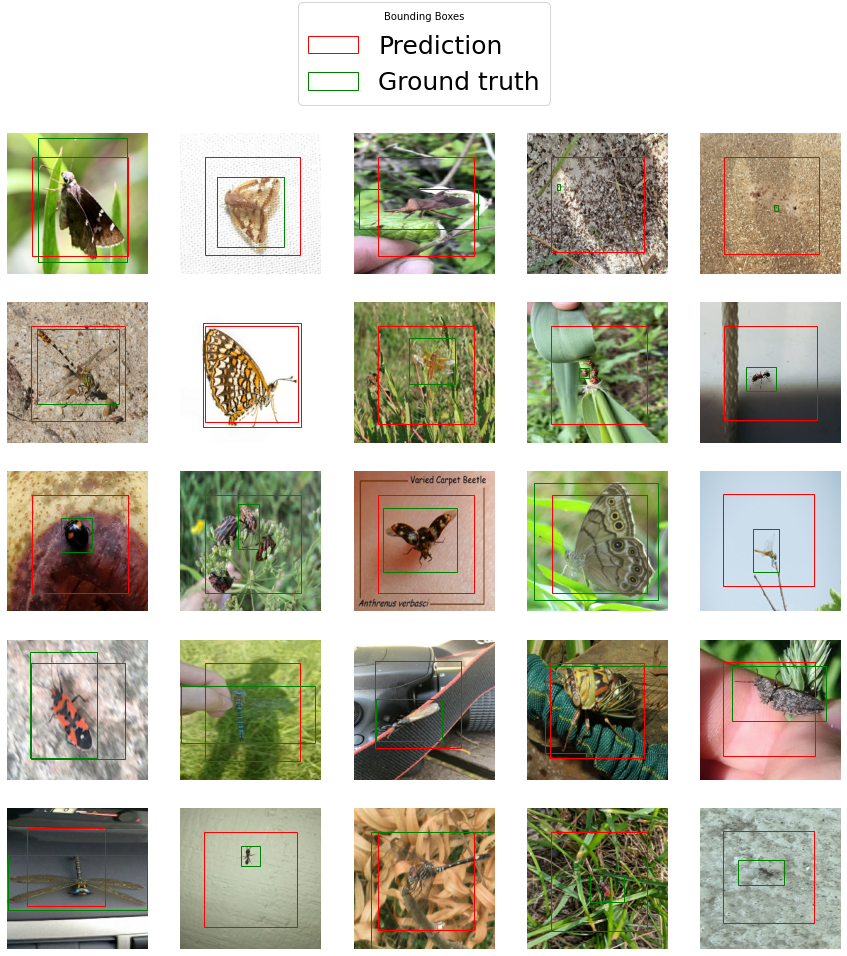
\includegraphics[width=\textwidth]{src/images/regression-inet.png}
        \end{minipage}
        \columnbreak
        \begin{minipage}{.45\textwidth}
            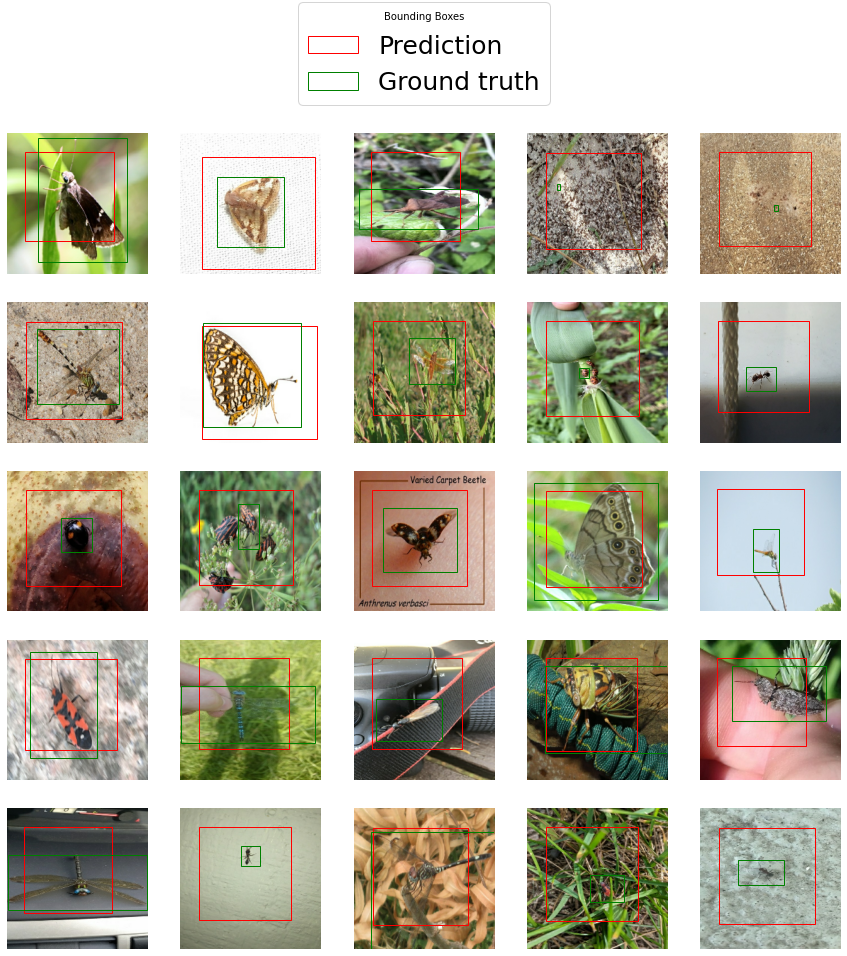
\includegraphics[width=\textwidth]{src/images/augmented-regression-inet.png}
        \end{minipage}
    \end{multicols}
    \begin{multicols}{2}
        \begin{minipage}{.45\textwidth}
            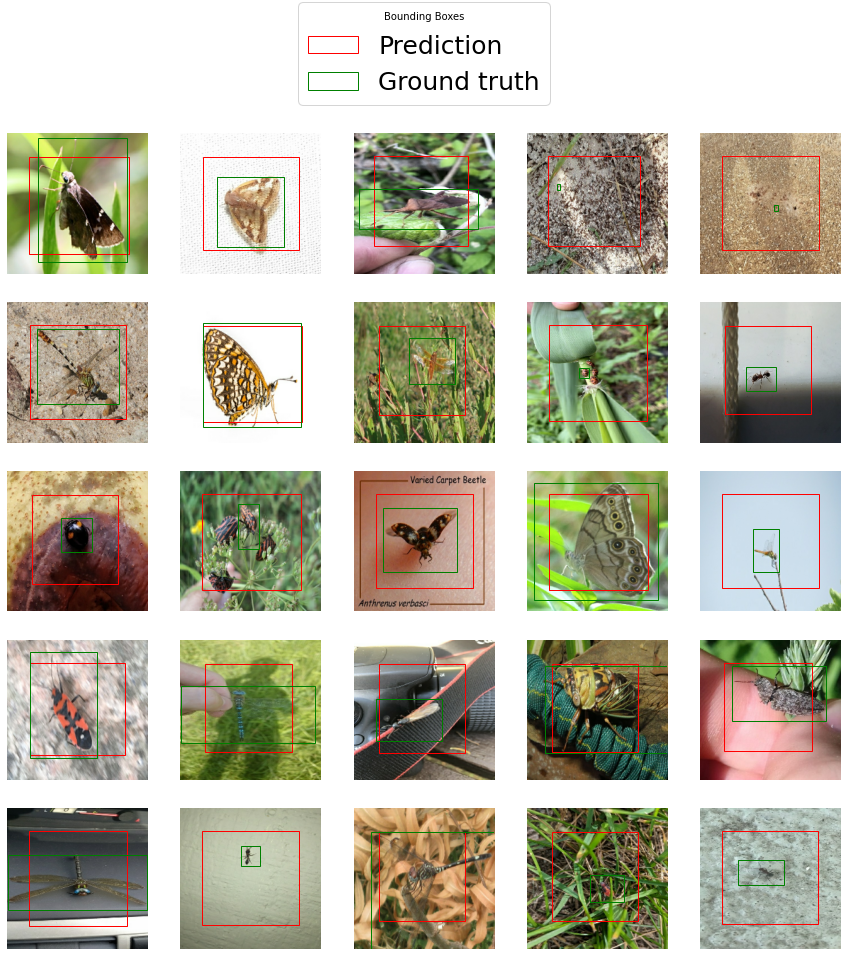
\includegraphics[width=\textwidth]{src/images/regression-mobilenet.png}
        \end{minipage}
        \columnbreak
        \begin{minipage}{.45\textwidth}
            \includegraphics[width=\textwidth]{src/images/augmented-regression-mobilenet.png}
        \end{minipage}
    \end{multicols}
    \begin{multicols}{2}
        \begin{minipage}{.45\textwidth}
            \includegraphics[width=\textwidth]{src/images/regression-vgg.png}
        \end{minipage}
        \columnbreak
        \begin{minipage}{.45\textwidth}
            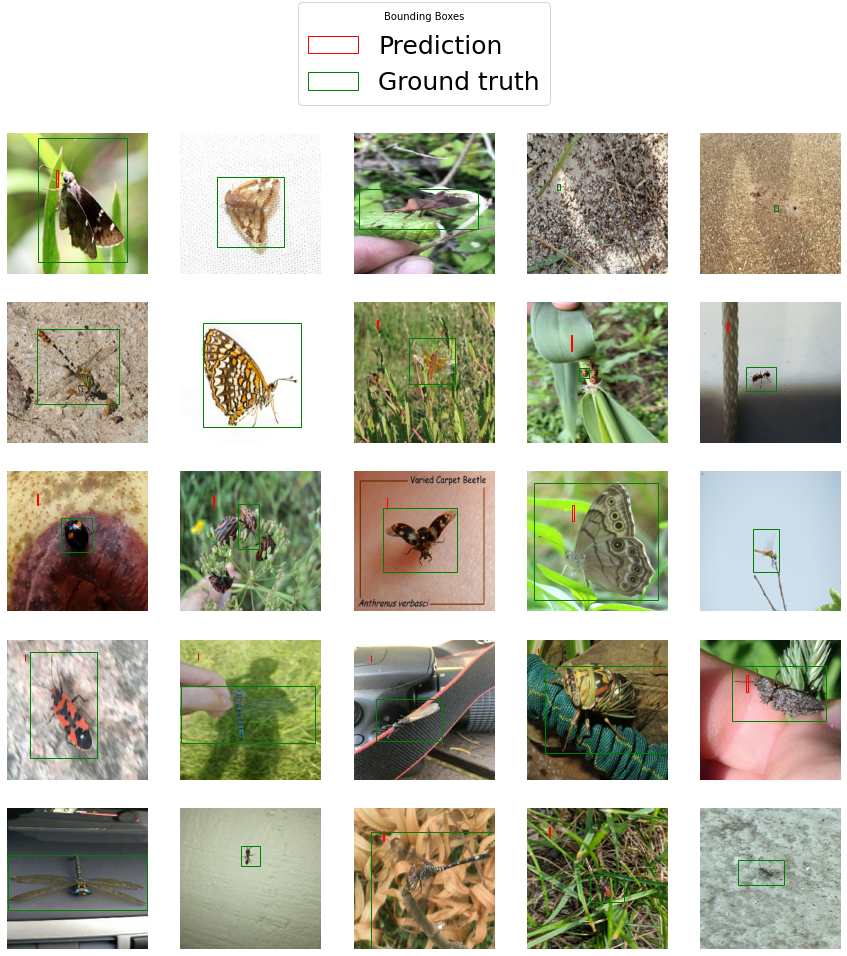
\includegraphics[width=\textwidth]{src/images/augmented-regression-vgg.png}
        \end{minipage}
    \end{multicols}
    \caption{Predictions of models solving the regression task. All predictions from the left column are from models trained on the original data set. The predictions on the right side are done by models trained on an augmented version of it.
    Starting from top, the first row contains predictions of INet based models, the second MobileNet, and the third by models based on VGG-16 as backbone.}
    \label{fig:regression-samples}
\end{figure}

\begin{figure}
    \centering
    \begin{multicols}{2}
        \begin{minipage}{.45\textwidth}
            \includegraphics[width=\textwidth]{src/images/classification-inet.png}
        \end{minipage}
        \columnbreak
        \begin{minipage}{.45\textwidth}
            \includegraphics[width=\textwidth]{src/images/augmented-classification-inet.png}
        \end{minipage}
    \end{multicols}
    \caption{Confusion matrix of predictions on the validation set for the model based on the INet backbone. Left trained on the cropped training (\eqref{eq:cropped-sample}) on the right side trained on the augmented version.
    The model trained on the raw data set seem to generalize better, compared to its counterpart trained on the augmented set.}
    \label{fig:classification-inet-conf}
\end{figure}
\begin{figure}
    \centering
    \begin{multicols}{2}
        \begin{minipage}{.45\textwidth}
            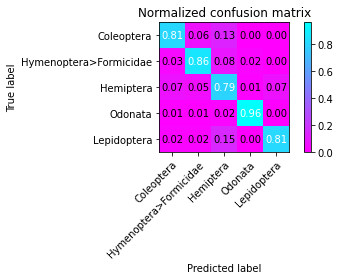
\includegraphics[width=\textwidth]{src/images/classification-mobilenet.png}
        \end{minipage}
        \columnbreak
        \begin{minipage}{.45\textwidth}
            \includegraphics[width=\textwidth]{src/images/augmented-classification-mobilenet.png}
        \end{minipage}
    \end{multicols}
    \caption{CMs for MobileNet classifier trained on the raw training set (left) and on the augmented version of it (right).
    Both models perform more or less equally on the validation set, but the overall predictive confidence of the left model seems to be higher than the right one.}
    \label{fig:classification-mobilenet-conf}
\end{figure}
\begin{figure}
    \centering
    \begin{multicols}{2}
        \begin{minipage}{.45\textwidth}
            \includegraphics[width=\textwidth]{src/images/classification-vgg.png}
        \end{minipage}
        \columnbreak
        \begin{minipage}{.45\textwidth}
            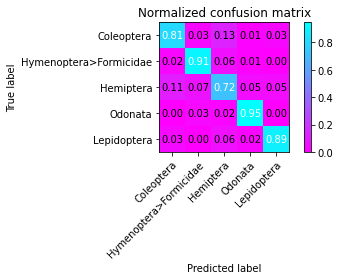
\includegraphics[width=\textwidth]{src/images/augmented-classification-vgg.png}
        \end{minipage}
    \end{multicols}
    \caption{Confusion matrices for VGG-16 trained on a raw (left) and an augmented (right) training set. Other than previous models, e.g. INet, VGG-16 seems to generalize better on augmented data.}
    \label{fig:classification-vgg-conf}
\end{figure}

\begin{figure}
    \centering
    \begin{multicols}{2}
        \begin{minipage}{.45\textwidth}
         \includegraphics[width=\textwidth]{src/images/uncropped-inet.png}
        \end{minipage}
        \columnbreak
        \begin{minipage}{.45\textwidth}
           \includegraphics[width=\textwidth]{src/images/sequential-classification-mobilenet.png}
        \end{minipage}
    \end{multicols}
    \caption{Confusion matrices for classification using a model having MobileNet as backbone and performing a specific task. Left the model was trained on uncropped images \eqref{eq:classification-sample} and will be used for the independent method approach. On the right side the model later used for the sequential method, trained on a training set generated using predictions of the best BBReg model.}
    \label{fig:extra-classification-mobilenet}
\end{figure}
\begin{figure}
    \centering
    \begin{multicols}{2}
        \begin{minipage}{.45\textwidth}
            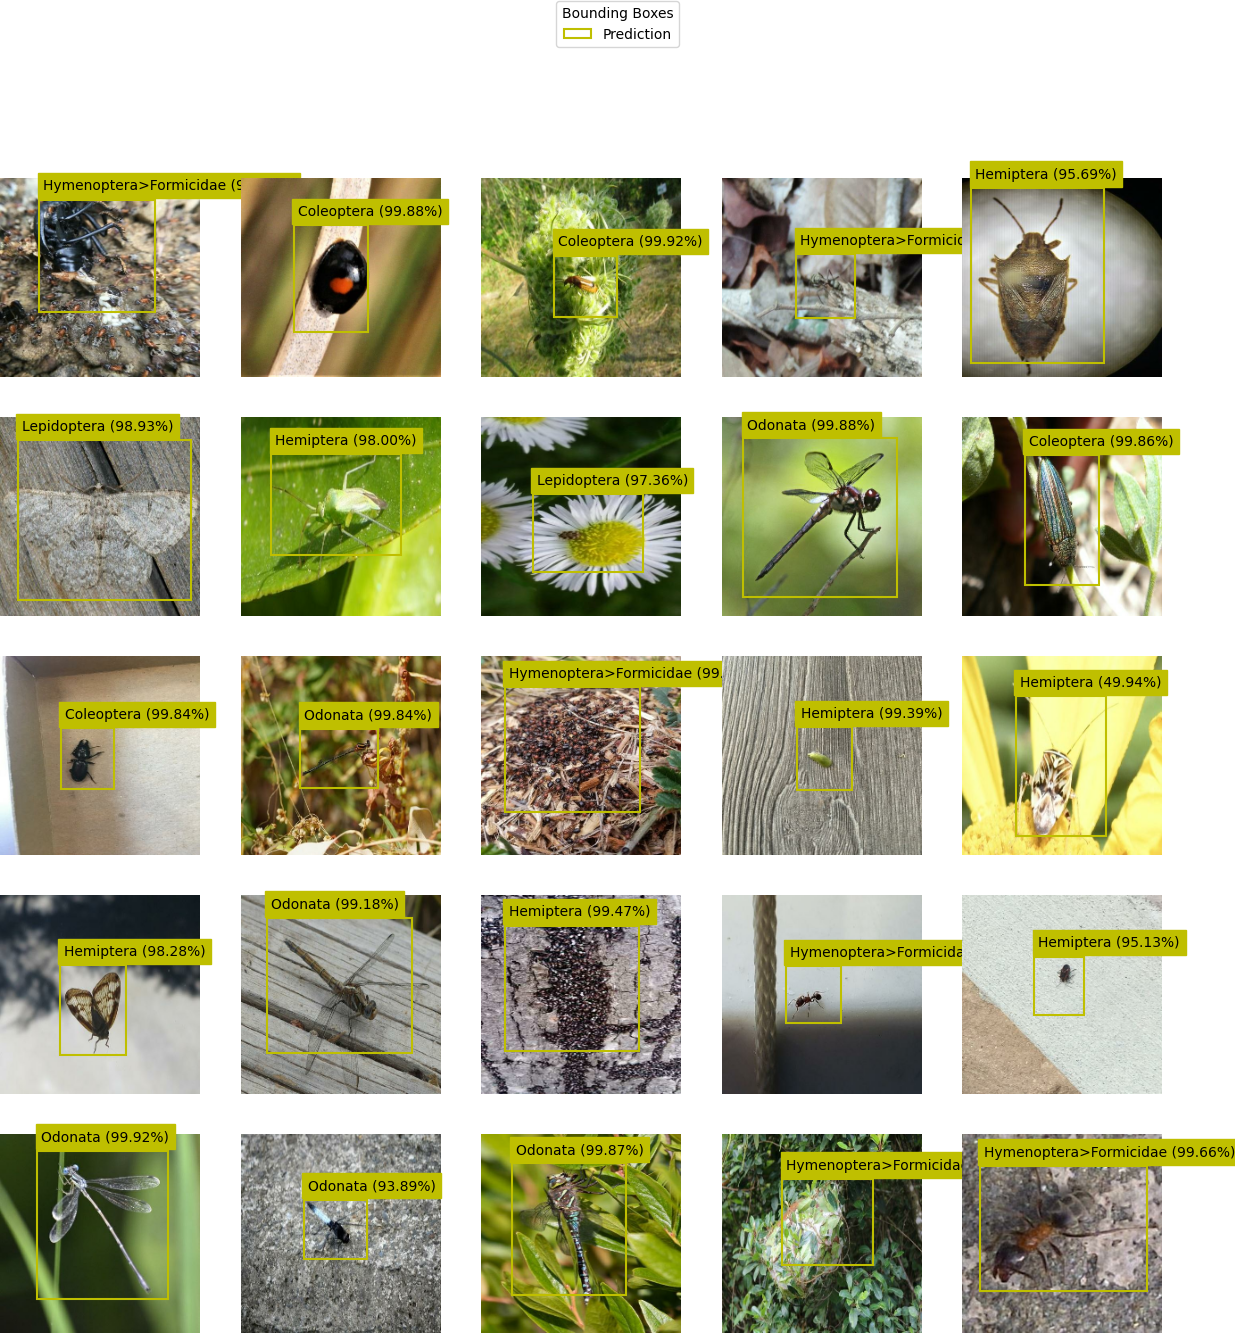
\includegraphics[width=\textwidth]{src/images/independent-model-predictions.png}
        \end{minipage}
        \columnbreak
        \begin{minipage}{.45\textwidth}
            \vspace{20pt}
            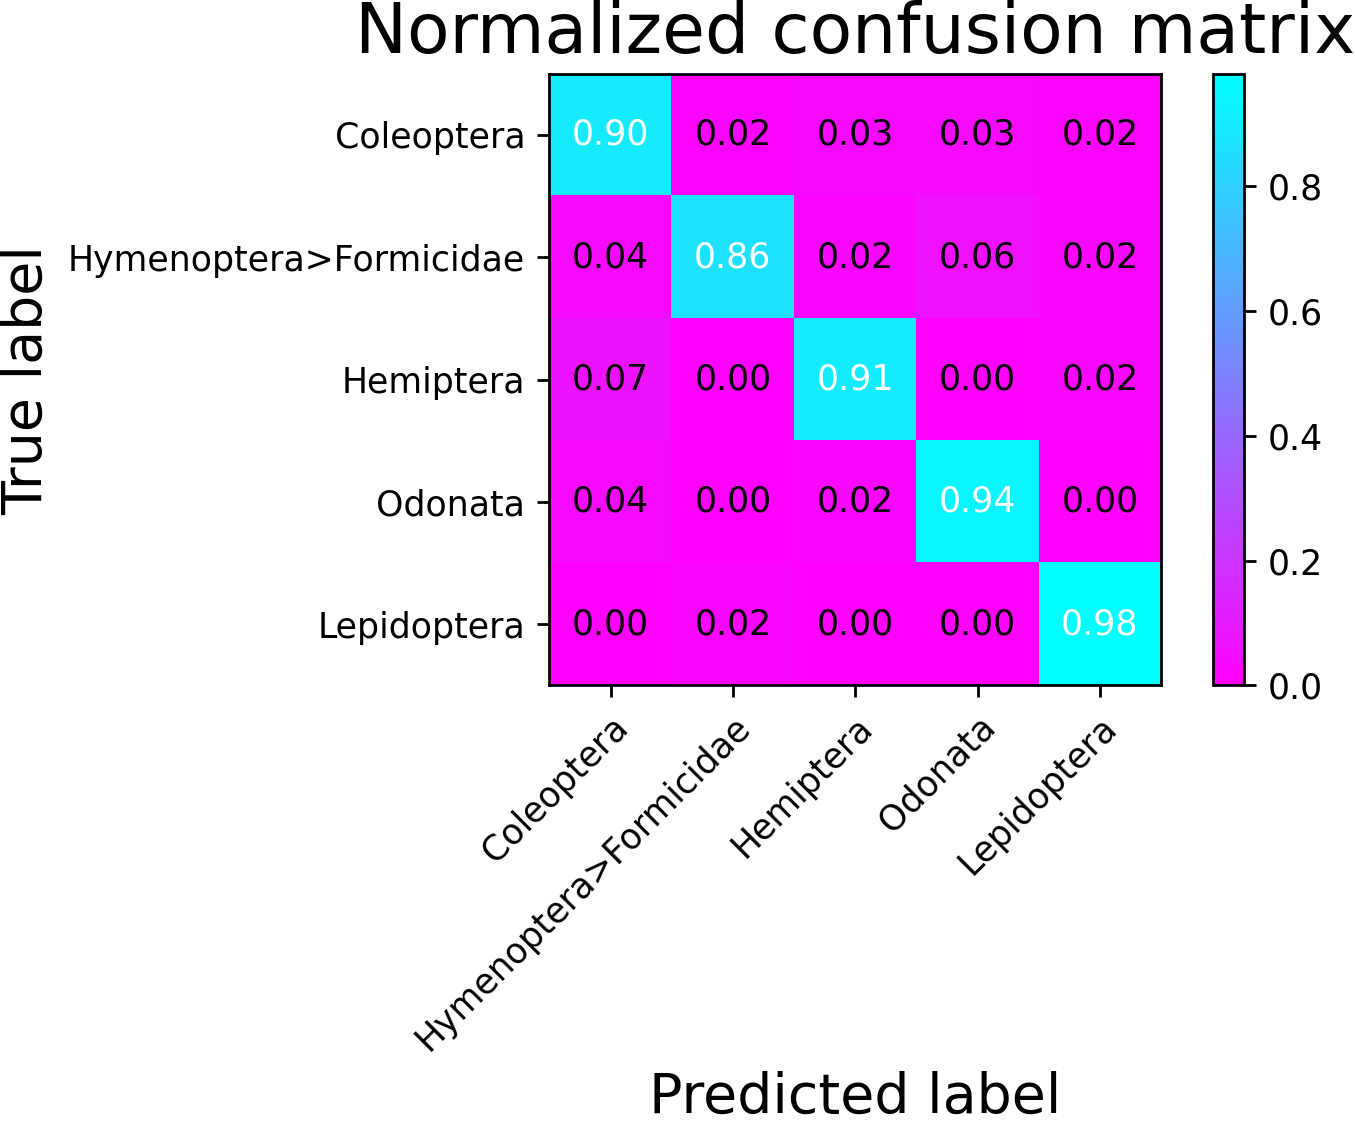
\includegraphics[width=\textwidth]{src/images/independent-model-confusion.png}
        \end{minipage}
    \end{multicols}
    \caption{Validation for independent two-stage-method. Left, predictions done by the solver on the test set, on the right side the related confusion matrix. The method seems to generalize well for the classification task, as the CM hints. The BBs generated by the method are good as well, but for some cases (row: 2, column: 3) the predictions are not very accurate.}
    \label{fig:independent-results}
\end{figure}
\begin{figure}
    \centering
    \begin{multicols}{2}
        \begin{minipage}{.45\textwidth}
            \includegraphics[width=\textwidth]{src/images/two-stage-model-predictions.png}
        \end{minipage}
        \columnbreak
        \begin{minipage}{.45\textwidth}
            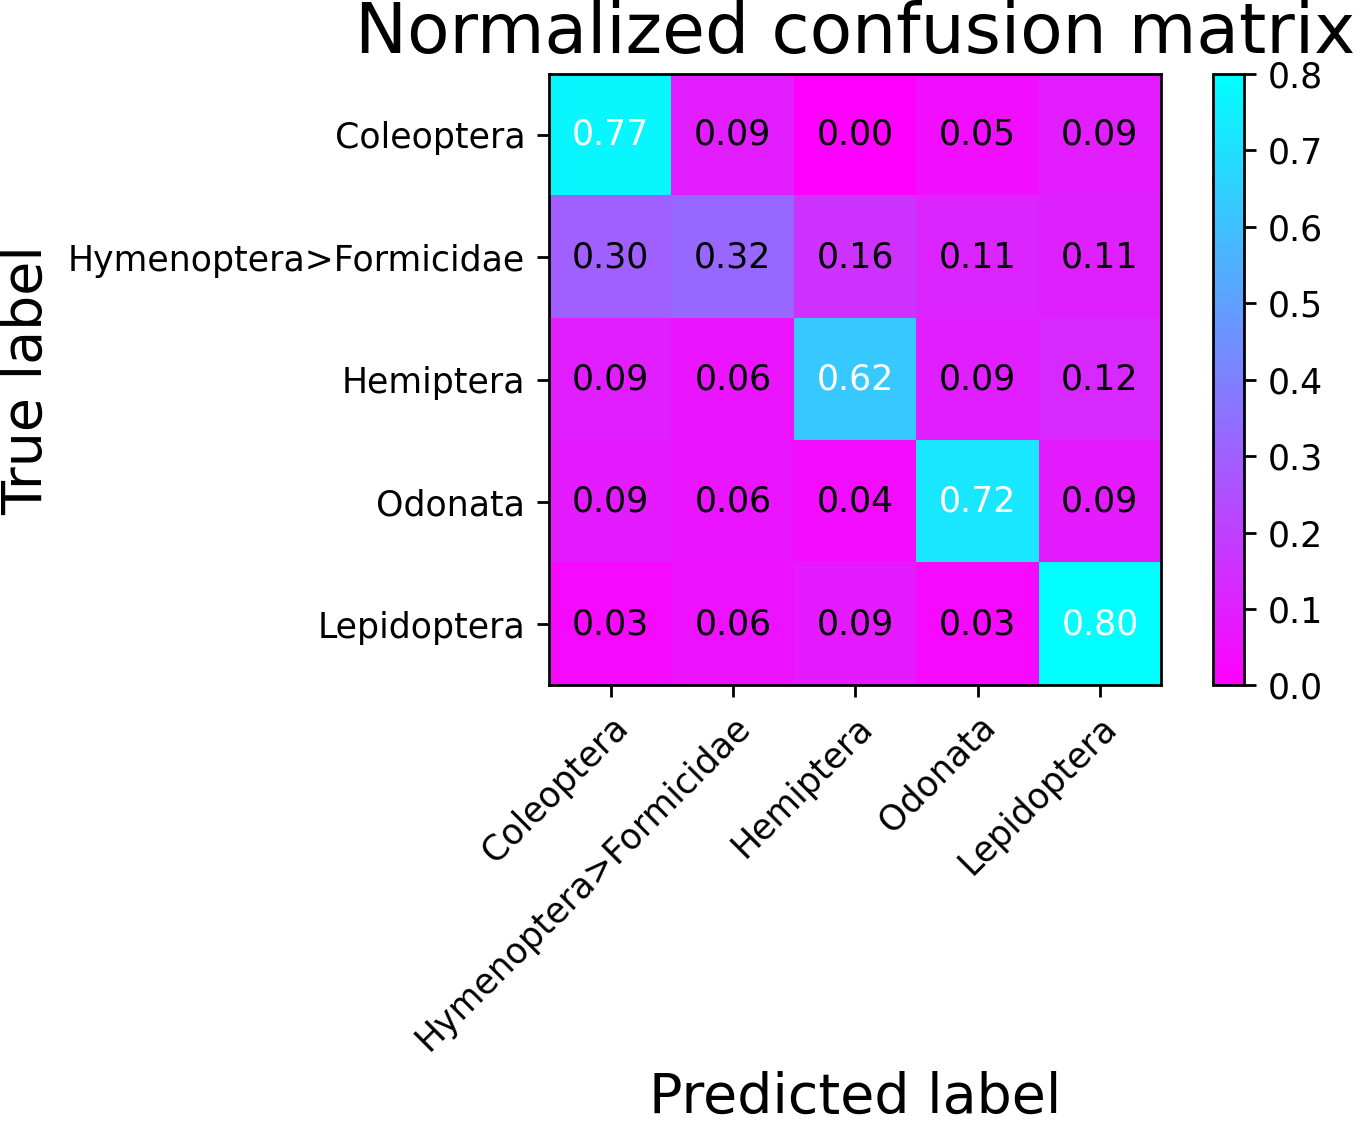
\includegraphics[width=\textwidth]{src/images/two-stage-model-confusion.png}
        \end{minipage}
    \end{multicols}
    \caption{Sequential two-stage-method validation. The BBs are the same as in \figref{fig:independent-results}. The confusion matrix differs. This is due to the fact that a new model was trained for the classification, but the regression task was solved by the same model. It seems that the sequential solver has trouble classifying Formicidae (ants).}
    \label{fig:sequential-results}
\end{figure}

\begin{figure}
    \centering
    \begin{multicols}{2}
        \begin{minipage}{.45\textwidth}
            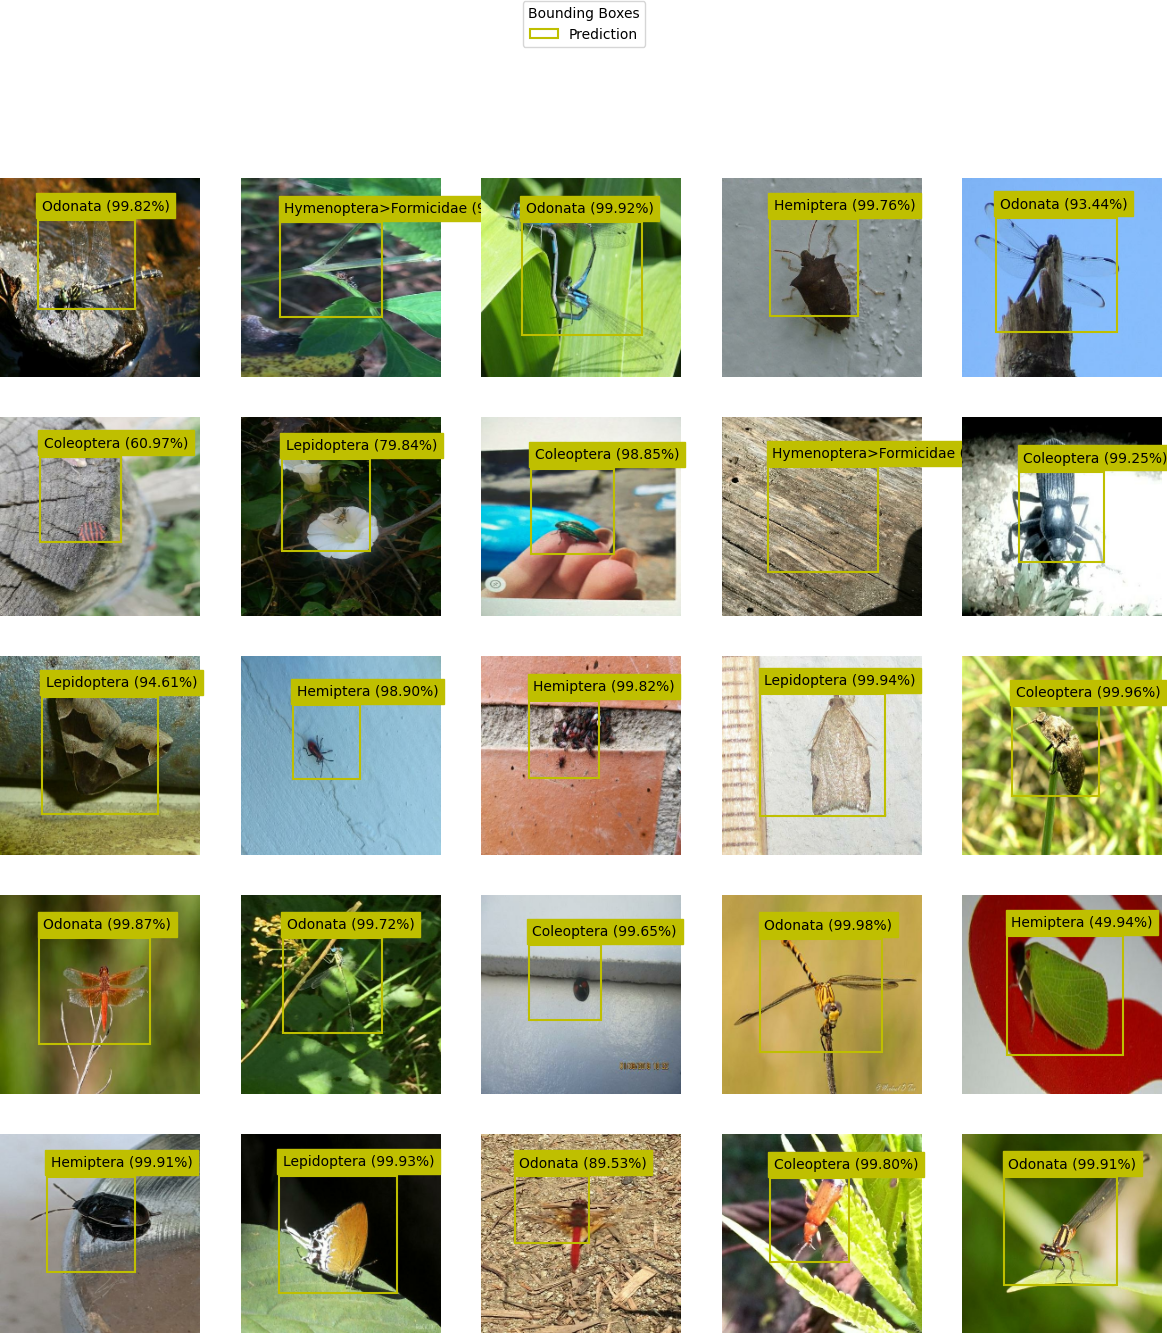
\includegraphics[width=\textwidth]{src/images/two-in-one-model-predictions.png}
        \end{minipage}
        \columnbreak
        \begin{minipage}{.45\textwidth}
            \includegraphics[width=\textwidth]{src/images/two-in-one-model-confusion.png}
        \end{minipage}
    \end{multicols}
    \caption{Evaluation of the single-stage-method, performed on the test set with samples of shape \eqref{eq:1-stage-sample}. The predictions on the left side show a problem, that was previously mentioned, the BBs seem to be fixed in one location. The results of the confusion matrix, compared to previous CMs (\figref{fig:independent-results} and \figref{fig:sequential-results}), more stable for all classes.}
    \label{fig:single-stage-predictions}
\end{figure}

\begin{figure}
    \centering
    \begin{multicols}{2}
        \begin{minipage}{.45\textwidth}
            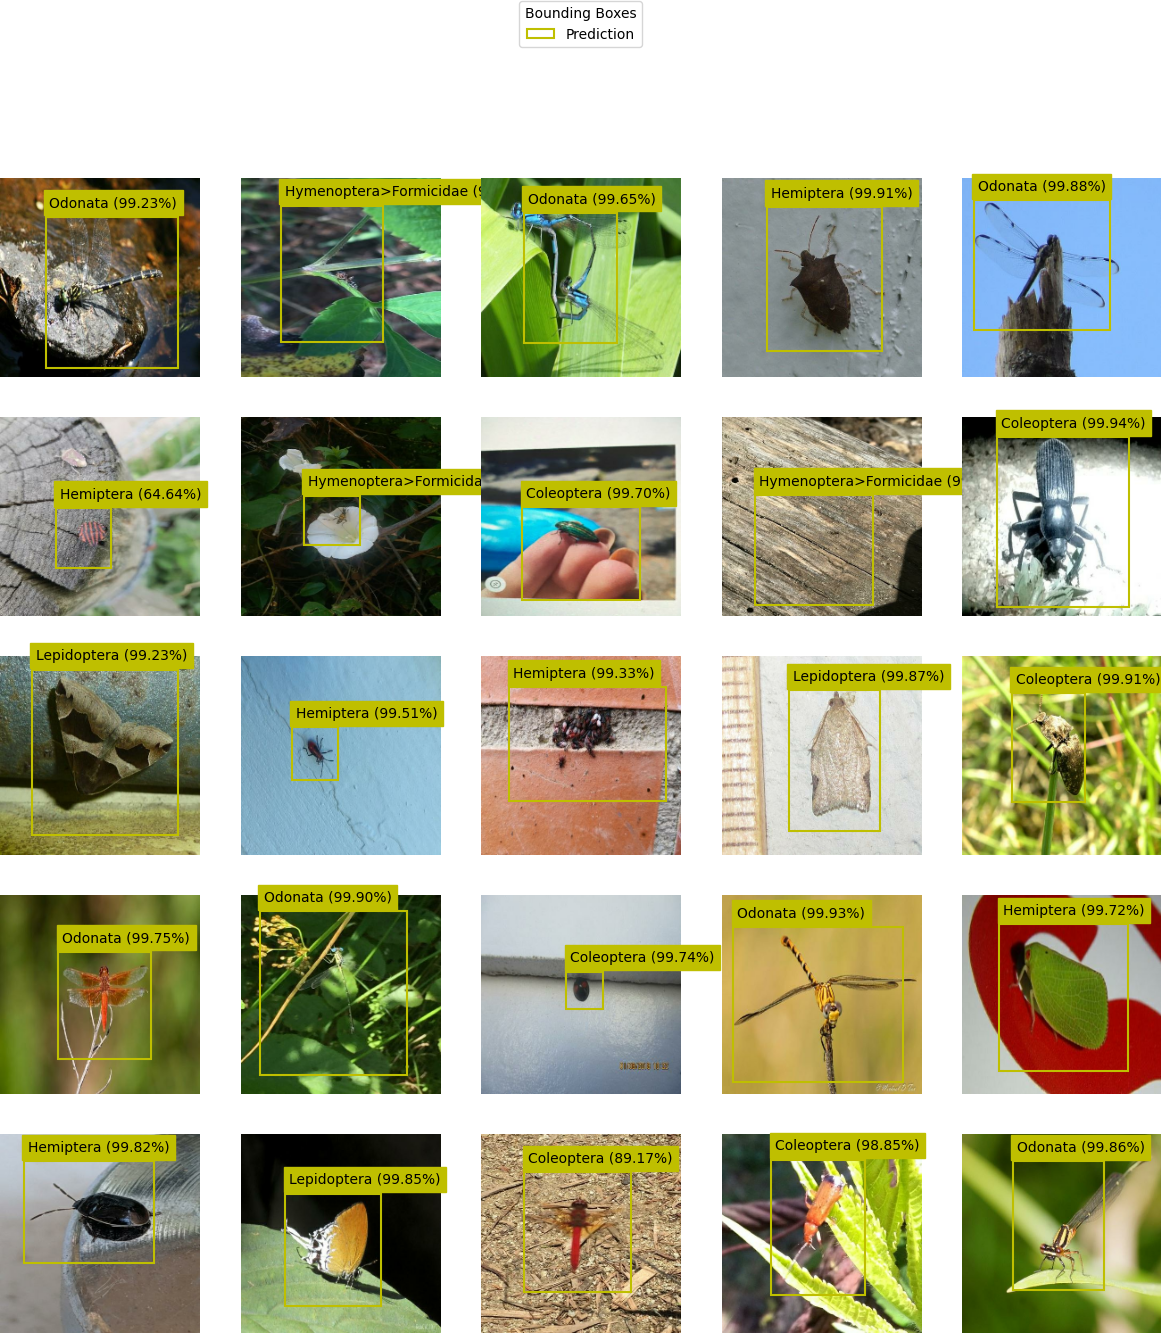
\includegraphics[width=\textwidth]{src/images/tf-lite-independent-model-predictions.png}
        \end{minipage}
        \columnbreak
        \begin{minipage}{.45\textwidth}
            \includegraphics[width=\textwidth]{src/images/tf-lite-independent-model-confusion.png}
        \end{minipage}
    \end{multicols}
    \caption{Validation results for TF Lite version of independent two-stage-method, using the test set. A decrease in quality for BB predictions, compared to its original model \figref{fig:independent-results}, was predictable due to the conversion to TF Lite. But the classification task does visually seem not to be solved in a less accurate way, this assumption is strengthened by the results displayed in \figref{fig:final-results-tflite}.}
    \label{fig:tflite-independent-results}
\end{figure}
\begin{figure}
    \centering
    \begin{multicols}{2}
        \begin{minipage}{.45\textwidth}
            \includegraphics[width=\textwidth]{src/images/tf-lite-two-stage-model-predictions.png}
        \end{minipage}
        \columnbreak
        \begin{minipage}{.45\textwidth}
            \includegraphics[width=\textwidth]{src/images/tf-lite-two-stage-model-confusion.eps}
        \end{minipage}
    \end{multicols}
    \caption{Results of validation for the sequential method converted to TF Lite applied to the test set. As in \figref{fig:tflite-independent-results} stated, the BB predictions decreased in quality. Unfortunately in this case the predictive decreased as well for the classification task, as the CM visualizes, e.g. the class Hemiptera lost $\approx 10\%$ in accuracy.}
    \label{fig:tflite-sequential-results}
\end{figure}

\begin{figure}
    \centering
    \begin{multicols}{2}
        \begin{minipage}{.45\textwidth}
            \includegraphics[width=\textwidth]{src/images/tf-lite-two-in-one-model-predictions.png}
        \end{minipage}
        \columnbreak
        \begin{minipage}{.45\textwidth}
            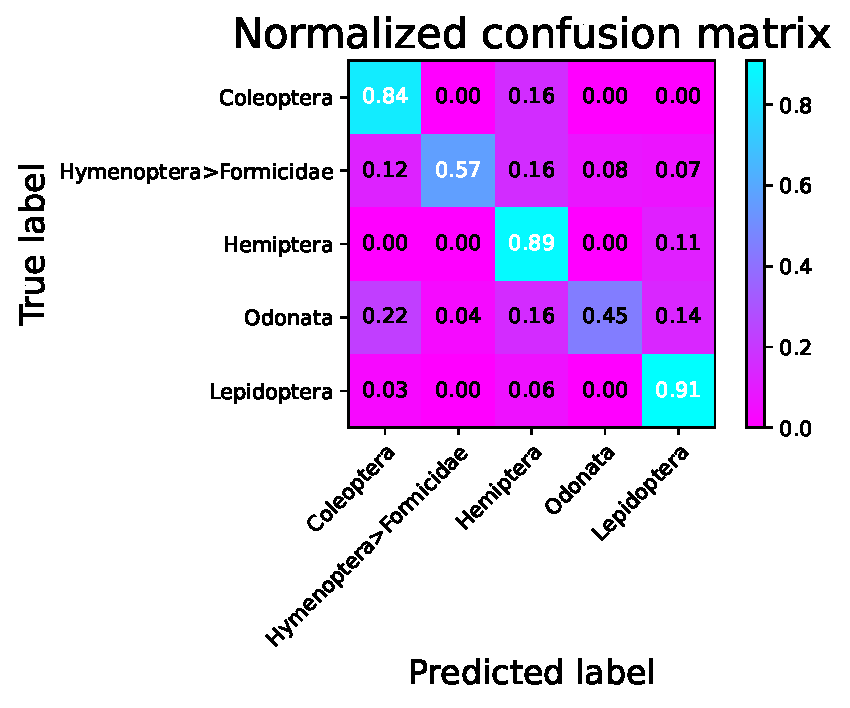
\includegraphics[width=\textwidth]{src/images/tf-lite-two-in-one-model-confusion.eps}
        \end{minipage}
    \end{multicols}
    \caption{Validation of the TF Lite version of the single-stage-method, based on the test set. The previously badly located (\figref{fig:single-stage-results}) decreased further in quality. Unfortunately, in this case also the classification quality decreases as listed in \figref{fig:final-results-tflite}. Whilst the original model performed well for the classification task, after converting to a TF Lite format the accuracy dropped drastically for all classes.}
    \label{fig:tflite-single-stage-results}
\end{figure}

\begin{figure}
    \centering
    \begin{multicols}{2}
        \begin{minipage}{.45\textwidth}
            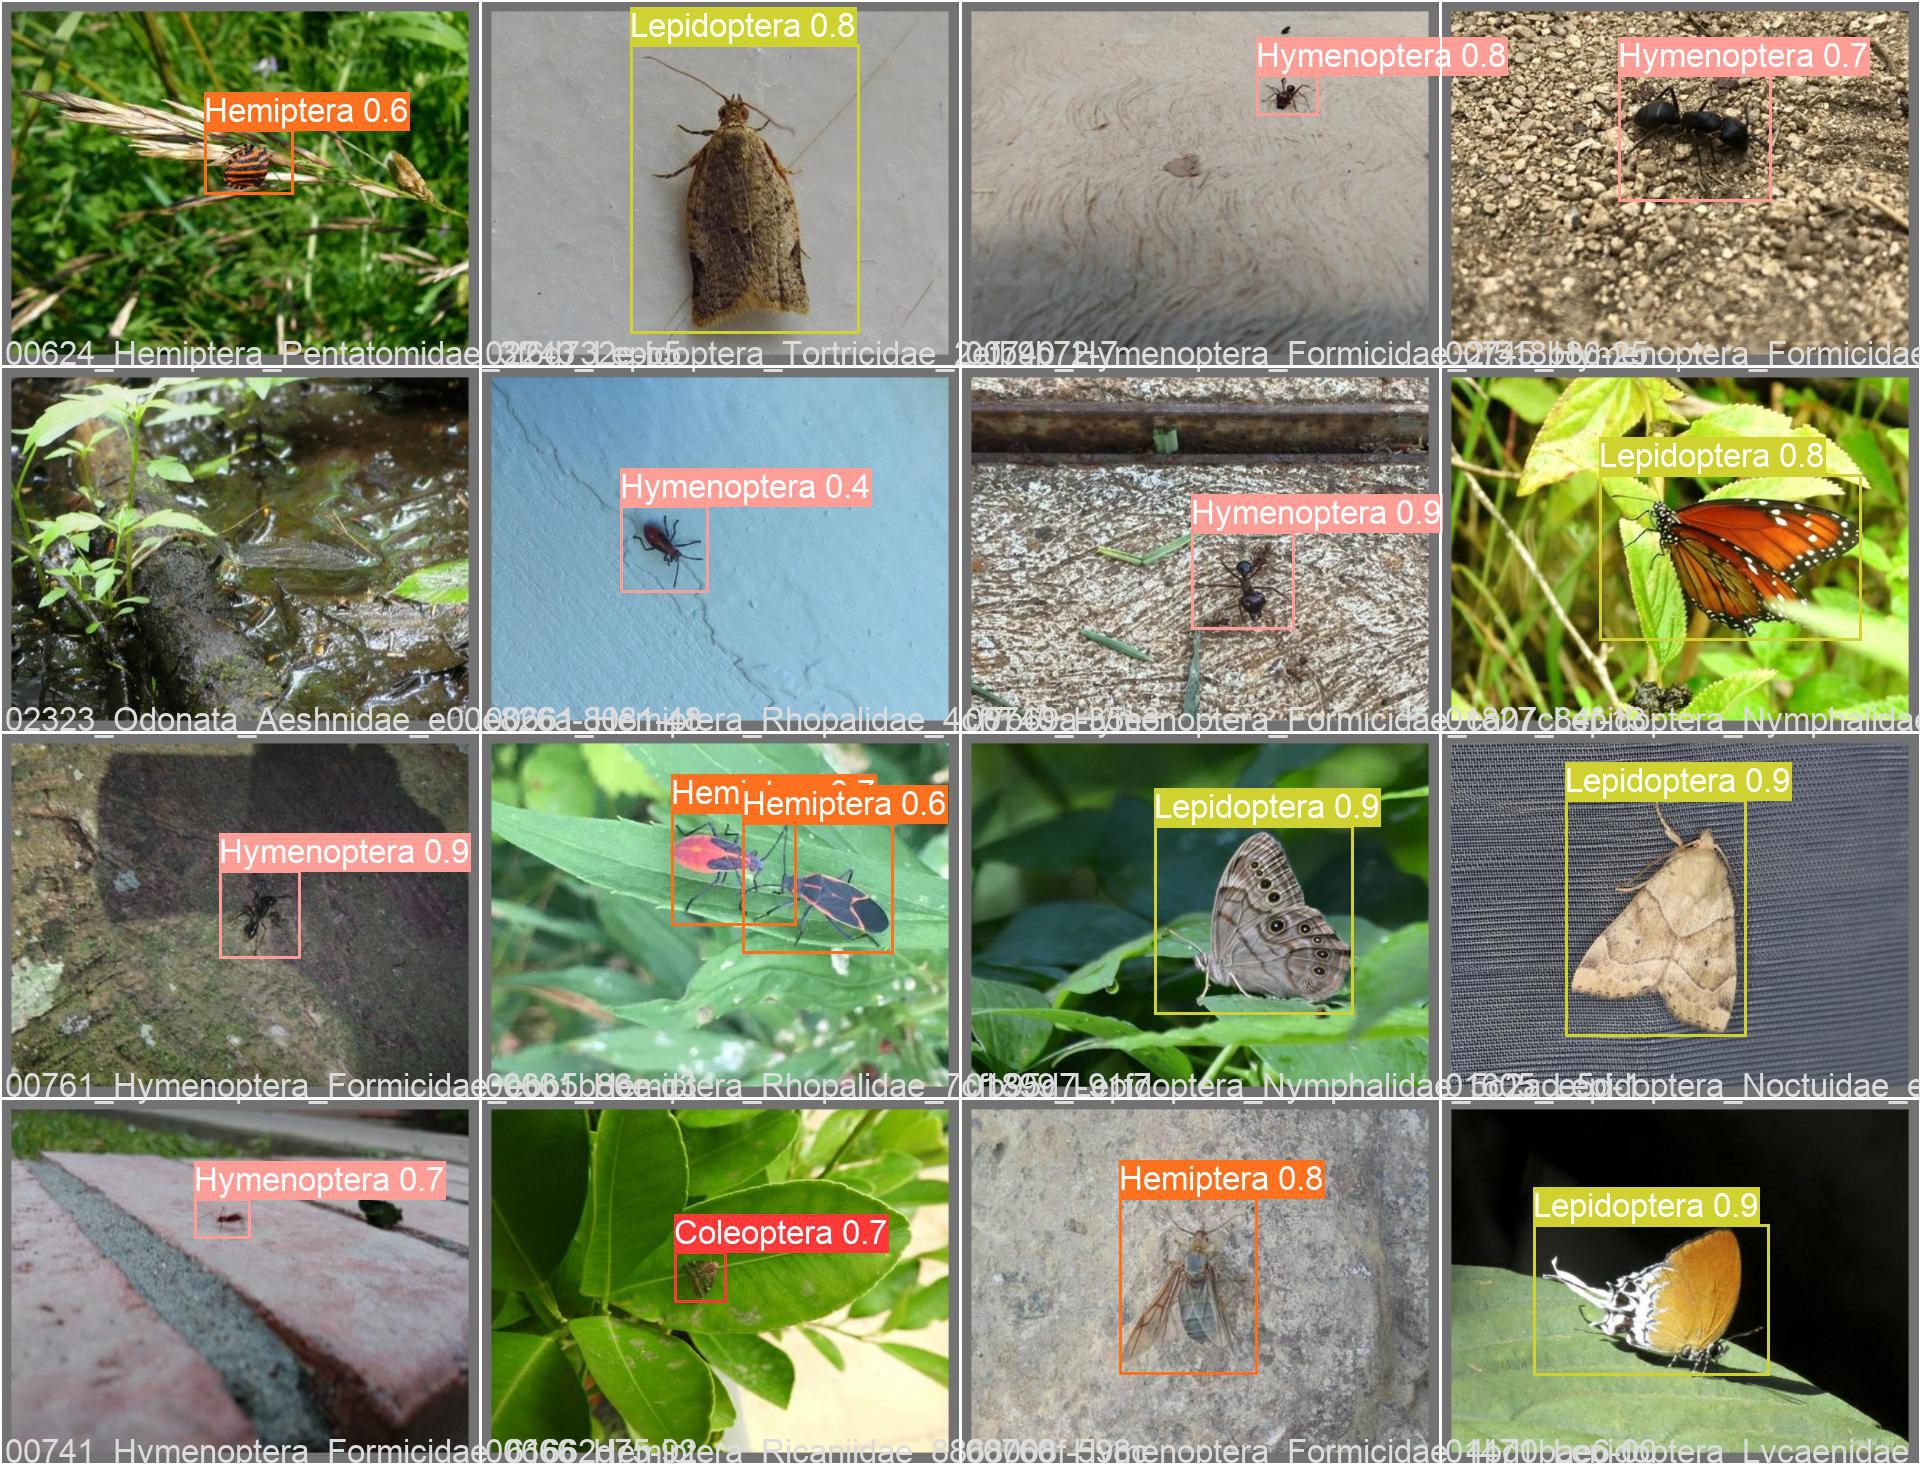
\includegraphics[width=\textwidth]{src/images/val_batch2_pred.png}
        \end{minipage}
        \columnbreak
        \begin{minipage}{.45\textwidth}
            \includegraphics[width=\textwidth]{src/images/yolo-confusion_matrix.png}
        \end{minipage}
    \end{multicols}
    \caption{Validation results for YOLOv5 converted to TF Lite. Left the previously displayed (\figref{fig:yolo-predictions}) predictions on the right side the related CM.}
    \label{fig:yolo-validation-results}
\end{figure}
